\documentclass[modern, letterpaper]{aastex62}

% to-do list
% ----------
% - write a first draft of the introduction
% - list our assumptions for detection & characterization (TheJoker)
% - Check abstract numbers (~80,000 RG stars with 3 or more good visits?)

% style notes
% -----------
% - This file generates by Makefile; don't be typing ``pdflatex'' or some BS.
% - Line break between sentences to make the git diffs readable.
% - Use \, as a multiply operator.
% - Reserve () for function arguments; use [] or {} for outer shit.
% - Always prior pdf or posterior pdf, never prior or posterior (that's your
%   arse).
% - Use \sectionname not Section, \figname not Figure, \documentname not Article
%   \tablename not Table, \eqname not Equation.
% - Make sure that two assumptions in the two assumption lists only have the
%   same name if they really are the same assumption: These are proper names!
% - Hyphenate binary-star when it is an adjective, not when it is a noun!
% - Where there are defined math symbols (like \pars), use them!

% other notes
% -----------
% - Binary engulfment reference: https://arxiv.org/pdf/1002.2216.pdf

\include{gitstuff}
% Load common packages
% \usepackage{microtype}  % ALWAYS!
\usepackage{amsmath}
\usepackage{amsfonts}
\usepackage{amssymb}
\usepackage{booktabs}

\usepackage{graphicx}
\usepackage{color}

\definecolor{cbblue}{HTML}{3182bd}
\usepackage{hyperref}
\definecolor{linkcolor}{rgb}{0.02,0.35,0.55}
\definecolor{citecolor}{rgb}{0.45,0.45,0.45}
\hypersetup{colorlinks=true,linkcolor=linkcolor,citecolor=citecolor,
            filecolor=linkcolor,urlcolor=linkcolor}
\hypersetup{pageanchor=true}

\newcommand{\documentname}{\textsl{Article}}
\newcommand{\sectionname}{Section}
\renewcommand{\figurename}{Figure}
\newcommand{\eqname}{Equation}
\renewcommand{\tablename}{Table}

% Packages / projects / programming
\newcommand{\package}[1]{\textsl{#1}}
\newcommand{\acronym}[1]{{\small{#1}}}
\newcommand{\github}{\package{GitHub}}
\newcommand{\python}{\package{Python}}
\newcommand{\emcee}{\project{emcee}}

% Missions
\newcommand{\project}[1]{\textsl{#1}}

% For referee
\newcommand{\changes}[1]{{\color{red} #1}}

% Stats / probability
\newcommand{\given}{\,|\,}
\newcommand{\norm}{\mathcal{N}}

% Maths
\newcommand{\dd}{\mathrm{d}}
\newcommand{\transpose}[1]{{#1}^{\mathsf{T}}}
\newcommand{\inverse}[1]{{#1}^{-1}}
\newcommand{\argmin}{\operatornamewithlimits{argmin}}
\newcommand{\mean}[1]{\left< #1 \right>}

% Unit shortcuts
\newcommand{\msun}{\ensuremath{\mathrm{M}_\odot}}
\newcommand{\kms}{\ensuremath{\mathrm{km}~\mathrm{s}^{-1}}}
\newcommand{\pc}{\ensuremath{\mathrm{pc}}}
\newcommand{\kpc}{\ensuremath{\mathrm{kpc}}}
\newcommand{\kmskpc}{\ensuremath{\mathrm{km}~\mathrm{s}^{-1}~\mathrm{kpc}^{-1}}}

% Misc.
\newcommand{\bs}[1]{\boldsymbol{#1}}
\definecolor{mahogany}{RGB}{165,15,21}
\newcommand{\resp}[1]{{\color{mahogany}#1}}

% Astronomy
\newcommand{\DM}{{\rm DM}}
\newcommand{\feh}{\ensuremath{{[{\rm Fe}/{\rm H}]}}}
\newcommand{\df}{\acronym{DF}}

% TO DO
\newcommand{\todo}[1]{{\color{red} TODO: #1}}


% adjust AAS-TEX shit
% \setlength{\parindent}{1.1\baselineskip}

\graphicspath{{figures/}}

% define macros for text
\newcommand{\apogee}{\project{\acronym{APOGEE}}}
\newcommand{\sdssiv}{\project{\acronym{SDSS-IV}}}
\newcommand{\thejoker}{\project{The~Joker}}
\newcommand{\thecannon}{\project{The~Cannon}}
\newcommand{\DR}{\acronym{DR14}}
\newcommand{\RC}{\acronym{RC}}
\newcommand{\RGB}{\acronym{RGB}}

\newcommand{\nRC}{XX}
\newcommand{\nRGB}{XX}
\newcommand{\ntotal}{XX}
\newcommand{\ncompanions}{XX}

% define macros for math
\newcommand{\hyperpars}{\gamma}
\newcommand{\pars}{\theta}

% for response to referee
% \renewcommand{\resp}[1]{#1}

\shortauthors{Price-Whelan et al.}

\begin{document}\sloppy\sloppypar\raggedbottom\frenchspacing % trust me

\title{Binary companions of red giant stars with APOGEE: \\
       catalog and companions that survive the common envelope}

\author[0000-0003-0872-7098]{Adrian~M.~Price-Whelan}
\affiliation{Department of Astrophysical Sciences,
             Princeton University, Princeton, NJ 08544, USA}
\email{adrn@astro.princeton.edu}
\correspondingauthor{Adrian M. Price-Whelan}

\author[0000-0003-2866-9403]{David~W.~Hogg}
\affiliation{Max-Planck-Institut f\"ur Astronomie,
             K\"onigstuhl 17, D-69117 Heidelberg, Germany}
\affiliation{Center for Cosmology and Particle Physics,
             Department of Physics,
             New York University, 726 Broadway,
             New York, NY 10003, USA}
\affiliation{Center for Data Science,
             New York University, 60 Fifth Ave,
             New York, NY 10011, USA}
\affiliation{Flatiron Institute,
             Simons Foundation,
             162 Fifth Avenue,
             New York, NY 10010, USA}

\author{Hans-Walter~Rix}
\affiliation{Max-Planck-Institut f\"ur Astronomie,
             K\"onigstuhl 17, D-69117 Heidelberg, Germany}

% \author{Jason~Cao}
% \affiliation{Center for Cosmology and Particle Physics,
%              Department of Physics,
%              New York University, 726 Broadway,
%              New York, NY 10003, USA}

\begin{abstract}\noindent % trust me
% Context
Repeat radial-velocity measurements of stars can be used to identify stellar-,
sub-stellar, and planetary-mass companions.
Even few observations are useful for detecting companions, though such data are
difficult to use for constraining physical properties because permitted orbital
solutions are highly degenerate.
% Aims
Here we perform a search for secondary companions of stars observed by the
\apogee\ survey (\DR), which has measured multi-epoch ($\geq 3$) but sparse
radial velocities for close to 100,000 stars.
% Methods
We use a custom-built Monte Carlo sampler (\thejoker) to deliver (often highly
multi-modal) posterior beliefs about companion orbital parameters.
In some cases, where the primary-star masses are known, the mass-function
degeneracy is broken and the secondary-companion masses ($m_2\,\sin i$) can be
inferred.
% Results
We provide a catalog of \ncompanions\ companions for which the companion
properties can be confidently determined, along with posterior samplings for all
\ntotal\ stars in the parent sample.
\todo{We find differences between the companions around \RC\ and \RGB\
stars that are in/consistent with the theoretical prediction that
stellar companions should not survive the common-envelope \RGB\ phase.}
\todo{We additionally find trends in XX with chemical abundances.}

We compare the companion populations of red clump (\RC) versus \RGB\ stars at
similar surface gravity and temperature, and study the metallicity dependence
of companion properties.

\end{abstract}

\keywords{
  binaries:~spectroscopic
  ---
  methods:~data~analysis
  ---
  methods:~statistical
  ---
  planets~and~satellites:~fundamental~parameters
  ---
  surveys
  ---
  techniques:~radial~velocities
}

\section{Introduction} \label{sec:intro}

\todo{Intro is missing many citations}

Stars typically have companions. Main sequence stars in the solar neighborhood
more often appear in binary or multiple star systems rather than as solitary
stars (\citealt{ragavhan,tokovinin,todo}).
This is likely a generic outcome of star formation: turbulent fragmentation in
collapsing protostellar clouds tends to produce multiplets of stars within
length-scales comparable to their spheres of influence (e.g.,
\citealt{Raskutti:2016}).
Binary and multiple star systems are therefore of great interest in
astrophysics: the population of stars and their companions encodes information
about star formation processes (\citealt{todo}), stellar parameters and
evolution (\citealt{todo}), and the dynamics of multi-body systems
(\citealt{todo}).

% Even without stellar or sub-stellar companions, the vast majority of stars have
% planetary-mass companions (\citealt{todo}).
% \todo{Planetary systems are interesting because...blah}
% Differences between the population of stellar companions and that of
% planetary-mass companions likely relate directly to the different formation
% channels for these objects.

Most of what is known about stellar companions comes from studies of
main-sequence (MS) stars.
MS stars with companions have a large dynamic range of constituent and orbital
characteristics.
For example, binary stars have mass-ratios that span from $\approx 10^-3$
\todo{citation because this is made up} to 1, and have periods from days to
millions of years.
\todo{Describe distributions over these quantities}
\todo{multiplicity in general: abundance, numbers, etc.}
\todo{some other stats from Moe and Di Stefano}

Some evolved stars have special roles in well-studied exotic multiple systems
like dwarf novae or cataclysmic variables \todo{are those examples correct?},
but by-in-large, less is known about the population of companions to evolved
stars.

- Expect differences in evolved star pop. from main sequence populations:
  - mass loss
  - envelope -> engulfment?
- Current samples limited in dynamical range of chemical properties, location,
  age (local to sun)
- Brighter, but typically larger distances, direct imaging not feasible
- Eclipsing companions good, but low mass companions stars -> hard to find
  (giants are big)
- Need large sample of stars with time-domain spectroscopy

% For planetary companions of main sequence stars, \todo{}.
% - Some indication of trends (e.g., with metallicity) -> star and
%   planet formation processes

Time-domain radial-velocity measurements of stars contain information about
massive companions: even with two successive observations of a single star, a
difference in the measured radial velocities implies the existence of at least
one companion.
However, with few or imprecise radial-velocity measurements, the orbital
properties of the companion(s) are very poorly constrained (e.g.,
\citealt{Price-Whelan:2017}).
The vast majority of spectroscopic targets with repeat observations in the
largest (by number of objects) stellar spectroscopic surveys are often observed
just a few times with sparse, non-uniform phase coverage.
Most prior searches for companions using survey RV data have therefore
restricted their searches to only sources with many, high-precision epochs, so
that the orbital solution can be unambiguously determined (e.g.,
\citealt{Troup:2016}), or have used simple statistics computed from the data to
study multiplicity (e.g., ${\rm RV}_{\rm max} - {\rm RV}_{\rm min}$;
\citealt{Badenes:2017}).

If there are only a few radial-velocity measurements made per star, and the
companion spectrum is not observed, any measured radial-velocity values will be
consistent with many different combinations of (primary) orbital parameters
(period, amplitude, eccentricity, etc.).
To identify companions to the typical star observed in a spectroscopic survey,
we therefore face at least one major challenge: how, given a small number of
observations of a primary star, do we reliably obtain posterior information
about the binary-system properties?
In general, the likelihood function---and the posterior probability distribution
function (pdf) under any reasonable prior pdf---will be highly multimodal, and
many of the modes will have comparable integrated probability density.
For example, with just two radial-velocity measurements, a harmonic series of
period modes will exist in the likelihood function.

We have solved this problem previously, though with limitations (to be discussed
more below), with \thejoker\ (\citealt{Price-Whelan:2017}).
\thejoker\ is a Monte Carlo rejection sampler that is computationally expensive
but probabilistically righteous:
It delivers independent posterior pdf samples for single-companion binary
orbital parameters, given any number of radial-velocity measurements.
Here we use \thejoker\ to generate posterior pdf samples for stars observed by
the \apogee\ survey (see \sectionname~\ref{sec:data}; \citealt{Majewski:2015}).

The \apogee\ surveys primarily target red-giant-branch (\RGB) stars, which are
ideal for the study of single-line binary systems.
For one, because they are so luminous, they are unlikely (in general) to have
equally-bright companions, and their spectra are therefore well-approximated or
fit as single-line objects.
When this constraint is not met, \thejoker\ will in general fail, and a model
that fits for a mixture of stellar spectra is more appropriate (e.g.,
\citealt{Kareem}).
The subset of \RGB\ stars in the ``red clump'' (\RC) are even more powerful as
they are standard candles and have masses that can be estimated using
spectroscopy (using dredged-up elements; \citealt{Martig:2016,Ness:2016}).
With primary-star mass estimates, the binary-orbit fitting will return
$m_2\,\sin i$ (minimum mass) estimates for the secondary, and not just estimates
of the so-called ``binary mass function.''
Additionally, the \apogee\ pipelines (\citealt{Garcia-Perez:2016}) and also
\thecannon\ (\citealt{Ness:2015}) produce detailed abundance estimates for \RGB\
and \RC\ stars.
If there are causal relationships between chemical abundances and binary
companions---as are expected---these should be measurable.

By making cuts on this library of posterior pdf samples (described in detail in
\sectionname~\ref{sec:whatever}), we deliver a catalog of binary-star systems
from the \apogee\ survey \todo{with ... (tease some statistics)}.
We additionally highlight the subset of this catalog with \RC\ star primaries,
for which we can compute companion mass and pericentric distance.

\section{Data} \label{sec:data}

All data used in this work comes from the publicly-available data release 14
(\DR) of the \apogee\ survey (\citealt{apogeedr14}), a component of the Sloan
Digital Sky Survey IV (\sdssiv; \citealt{sdss,Blanton:2017}).
\apogee\ is an infrared spectroscopic survey designed to map \RGB\ stars across
much of the Milky Way.
Targets are selected with simple color and brightness cuts, but the survey uses
fiber-plugged plates with a maximum of \todo{100?} fibers and a $\approx
1.5~{\rm deg}^2$ field of view, leading to ``pencil-beam''-like sampling of the
stellar distribution.
Data taken as part of the \apogee\ survey is reduced with the \todo{APOGEE
spectral parameter...} (\acronym{ASPCAP}; \citealt{Garcia-Perez:2016}), which
measures stellar parameters, chemical abundances, and radial velocities for each
target.
\todo{talk about visits, how the velocities measured...}

We use the primary data products from \apogee\ \DR\ (i.e. the \texttt{allStar}
and \texttt{allVisit} files) which contain 258475 unique source IDs
(\texttt{APOGEE\_ID}) and 1054381 unique visits.
We select all stars with $\geq 3$ visits that each pass a set of quality cuts,
described below.
For each visit, we require that the visit velocity uncertainty is $< 100~\kms$
(\texttt{VRELERR}) and the following bits are not set in the \texttt{STARFLAGS}
bitmask: \texttt{PERSIST\_HIGH}, \texttt{PERSIST\_JUMP\_POS},
\texttt{PERSIST\_JUMP\_NEG}, \texttt{VERY\_BRIGHT\_NEIGHBOR}, \texttt{LOW\_SNR}.
For each star, we require that $0 < \log g < 3.5$ and the following bits are not
set in the \texttt{ASPCAPFLAGS} bitmask: \texttt{STAR\_BAD}.
After these cuts, and the requirement of $\geq 3$ visits for a given star, we
are left with \todo{XX} visits for \todo{XX} unique stars (unique
\texttt{APOGEE\_ID}).
\todo{add numpy code for exact filter?}
\figurename~\ref{fig:nvisits} shows the number of stars in several bins of
number of visits that pass the above quality cuts: \todo{XX}\% of the stars in
\DR\ have $< 8$ visits.

% Notebook: "Numbers after cuts"
\begin{figure}[hp]
\begin{center}
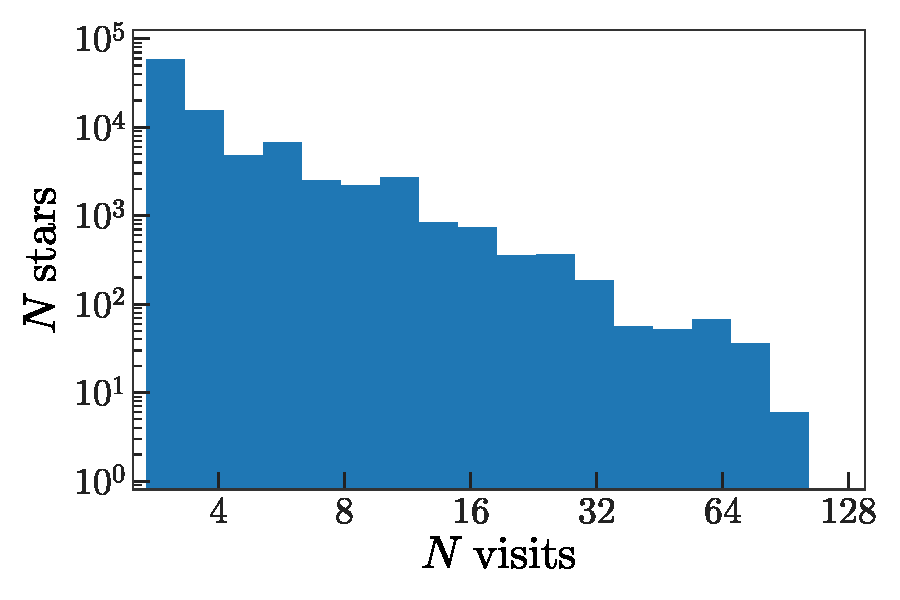
\includegraphics[width=\textwidth]{nvisits.pdf}
\end{center}
\caption{%
TODO: \label{fig:nvisits}
}
\end{figure}


\section{Methods}

\subsection{Orbit fitting and velocity modeling}\label{sec:fitting}

For every source in the sample of \apogee\ stars defined in
\sectionname~\ref{sec:data}, we obtain a posterior sampling in binary-system
parameter space, treating it as a single-lined (SB1) spectroscopic binary system
with a single companion.
This sampling is performed under a relatively uninformative prior pdf, and the
resulting posterior samplings are used to discover and characterize individual
binary-star systems and generate a catalog of companions.
We use \thejoker\ to perform the posterior samplings; we briefly describe the
algorithm below, but a full description is given in previous work
(\citealt{Price-Whelan:2017}).
In this \sectionname, we describe the assumptions and method used to generate
individual-system samplings.

We perform our individual system fits---that is, make our posterior
samplings---under the following assumptions:
\begin{description}
\item[no multiplets] All radial-velocity variations of the primary star are
  induced by a single companion.
  This is motivated by the idea that triple star systems are usually
  hierarchical so that the period of the inner binary is typically much shorter
  than the orbital period of the outer body (\todo{CITATION NEEDED}).
  At present, we ignore the possibility of higher-order multiple systems.
  \todo{revisit this - do we want to also sample over a long-term trend?}
\item[Kepler] Related to the first point, all velocity variations of the primary
  are gravitational, and we therefore ignore the possibility of intrinsic
  variation from, e.g., stellar oscillations.
\item[SB1] All spectra are single-lined; that is, we assume that the secondary
  is significantly fainter and is thus undetected in the spectra.
  This assumption is motivated by the fact that we expect \RGB\ stars to be
  substantially more luminous than their typical companion.
  However, there are known double-lined binary stars in the \apogee\ catalog
  (El-Badry et al., in prep.), and an unknown fraction of \RGB--\RGB\ binaries.
\item[simple noise model] Measurements are unbiased and noise estimates are
  correct up to an \todo{unknown} extra variance (the ``jitter'').
  All noise contributions result in Gaussian uncertainties on the individual
  radial-velocity measurements.
\end{description}

\thejoker\ is a custom-built Monte Carlo sampler designed to produce independent
posterior samples in orbital parameters, given radial-velocity measurements
under the assumptions above.
Our parametrization is similar to the notation in \citet{Murray:2010}:
The radial velocity $v$ at time $t$ is given by
\begin{equation}
  v(t;\bs{\theta}) = v_0 + K\,[\cos\left(\omega + f(t; e, P, \phi_0)\right) +
    e\,\cos\omega]
\end{equation}
where $\bs{\theta} = (P,e,\phi_0,\omega,K,v_0)$---period, eccentricity, initial
phase, argument of pericenter, velocity semi-amplitude, Barycentric velocity---
and the true anomaly, $f$, is a function of the specified parameters (see
\sectionname~2 of \citealt{Price-Whelan:2017} or \eqname~63 in
\citealt{Murray:2010}).

\thejoker\ was designed for the extremely multi-modal pdfs expected when the
number of radial-velocity measurements of a source is small, or the data have
low signal-to-noise.
While other Markov Chain Monte Carlo (MCMC) methods have difficulty producing
independent samples with such data, \thejoker\ succeeds by brute force.
After generating an initial (very large) library of prior samples from an
assumed prior pdf (see below), the (typically multi-modal) likelihood is
evaluated at each sample and used to rejection sample.
In practice, given a number of requested samples for each star, the sampling
proceeds iteratively: since it is easier to accept samples when the data is
sparse or noisy, far more prior sample draws (and thus likelihood
evaluations) must occur under very constraining data.

In addition to generating posterior samples for each source, we also compute the
fully marginalized likelihood (FML) under two other models: (1) a model in which
the radial velocity of the source is constant, and (2) a model in which the
radial-velocity variations are purely linear.
We later use these FML values to define cuts on our full catalog of posterior
samples to produce a catalog of companions.

\todo{equations?}

Examples of outputs and etc.

\subsection{Infer the jitter}

For each $n$ of $N$ RGB stars in APOGEE, we obtain $K$ posterior samples over
primary orbital parameters $\bs{w} = (P, e, \omega, \phi_0, K, v_0)$ and the
jitter parameter, $y = \ln s^2$, using \textit{The Joker}.
To obtain this sampling, we use an interim prior on the jitter parameter
parametrized by a mean and root-variance $\alpha_0 = (\mu_{y,0}, \sigma_{y,0})$.

\begin{eqnarray}
    \bs{\theta}_{k} &=& (\bs{w}, y)_{k}\\
    \bs{\theta}_{k} &\sim& p(\bs{\theta}_k \given \{D_n\}, \alpha_0)
\end{eqnarray}

New hyperprior, parameters to infer: $\alpha = (\mu_y, \sigma_y)$.

We want to obtain posterior samples in
\begin{eqnarray}
    p(\alpha \given \{D_n\}) &\propto& p(\{D_n\} \given \alpha) \, p(\alpha)
\end{eqnarray}
where
\begin{eqnarray}
    p(\{D_n\} \given \alpha) &=& \prod_n^N p(D_n \given \alpha) \quad .
\end{eqnarray}


\begin{eqnarray}
    p(D_n \given \alpha) &=& \int \dd \theta_n \, p(D_n \given \theta_n) \,
      p(\theta_n \given \alpha)\\
    &=& \int \dd \theta_n \, p(D_n \given \theta_n) \, p(\theta_n \given \alpha) \,
      \frac{p(\theta_n \given D_n, \alpha_0)}{p(\theta_n \given D_n, \alpha_0)}\\
    &=& \int \dd \theta_n \, p(D_n \given \theta_n) \, p(\theta_n \given \alpha) \,
      p(\theta_n \given D_n, \alpha_0) \,
      \frac{p(D_n \given \alpha_0)}{p(D_n \given \theta_n) \,
      p(\theta_n \given \alpha_0)}\\
    &=& p(D_n \given \alpha_0) \, \int \dd \theta_n \,
      \frac{p(\theta_n \given \alpha)}{p(\theta_n \given \alpha_0)} \,
      p(\theta_n \given D_n, \alpha_0)\\
    &\approx& \mathcal{Z}_n \, \frac{1}{K_n} \,
      \sum_k^{K_n} \frac{p(\theta_{nk} \given \alpha)}{p(\theta_{nk} \given \alpha_0)}\\
    &=& \frac{\mathcal{Z}_n}{K_n} \,
      \sum_k^{K_n} \frac{p(y_{nk} \given \alpha)}{p(y_{nk} \given \alpha_0)}
\end{eqnarray}

\begin{eqnarray}
    p(\{D_n\} \given \alpha) &\propto& \prod_n^N \frac{1}{K_n} \,
      \sum_k^{K_n} \frac{p(y_{nk} \given \alpha)}{p(y_{nk} \given \alpha_0)}\\
    \ln p(\{D_n\} \given \alpha) &\propto& \sum_n^N \left[
      \ln\left( \sum_k^{K_n} \frac{p(y_{nk} \given \alpha)}{p(y_{nk} \given \alpha_0)} \right)
      - \ln K_n\right]\\
    &\propto& \sum_n^N \left[
      \underset{k}{\rm logsumexp}\left[ \ln{p(y_{nk} \given \alpha)} - \ln{p(y_{nk} \given \alpha_0)} \right]
      - \ln K_n\right]
\end{eqnarray}

\section{Results}

\subsection{Catalog / posterior samples whatever} \label{sec:full-catalog}

\todo{APW}

\subsection{A catalog of confident companions} \label{sec:conf-companions}

\todo{APW}

Thresholding on what now?

Catalog.

Some highlights from this catalog.

\subsection{Differences in companions of RC and RGB stars}
\label{sec:rc-rgb}

\todo{APW}

\subsection{Trends in RGB companions with chemical abundances}
\label{sec:rgb-chemistry}

\todo{APW}

\section{Discussion}

Return to our various assumptions and make sure that we discuss them
\emph{by name} here.

\acknowledgements

It is a pleasure to thank Keith Hawkins (Columbia), XXXXXXX.

The authors are pleased to acknowledge that the work reported on in this
paper was substantially performed at the TIGRESS high performance computer
center at Princeton University which is jointly supported by the Princeton
Institute for Computational Science and Engineering and the Princeton
University Office of Information Technology's Research Computing department.

\software{
The code used in this project is available from
\url{https://github.com/adrn/TwoFace} under the MIT open-source
software license.
This research utilized the following open-source \python\ packages:
    \package{Astropy} (\citealt{Astropy-Collaboration:2013}),
    % \package{corner} (\citealt{Foreman-Mackey:2016}),
    % \package{emcee} (\citealt{Foreman-Mackey:2013ascl}),
    \package{IPython} (\citealt{Perez:2007}),
    \package{matplotlib} (\citealt{Hunter:2007}),
    \package{numpy} (\citealt{Van-der-Walt:2011}),
    \package{scipy} (\url{https://www.scipy.org/}),
    \package{sqlalchemy} (\url{https://www.sqlalchemy.org/}).
}

\facility{\sdssiii, \apogee}

\bibliographystyle{aasjournal}
\bibliography{refs}

\end{document}
